\documentclass{sig-alternate-per-modified}

\usepackage[utf8]{inputenc}
%\usepackage[T1]{fontenc}
\usepackage{amsmath,amsfonts}
%\usepackage{array}
\usepackage{tikz, pgfplots}
\usepackage{mathtools, balance}
\usepackage{subfig}
% Circuit
\usepackage{cite}
% Notation
\usepackage{siunitx}
\usepackage{balance}
\usepackage{microtype}

% Theorems
\newtheorem{theorem}{Theorem}[section]
\newtheorem{proposition}[theorem]{Proposition}
\newtheorem{definition}[theorem]{Definition}
\newtheorem{corollary}[theorem]{Corollary}
\newtheorem{remark}[theorem]{Remark}
\newtheorem{assumption}[theorem]{Assumption}
\newtheorem{example}[theorem]{Example}
\newtheorem{lemma}[theorem]{Lemma}
%\newtheorem*{lemma*}{Lemma}

% Pgfplots
\pgfplotsset{width=\columnwidth, height = 0.75\columnwidth, grid style = {dashed, gray}, every tick label/.append style = {font=\footnotesize}, compat=1.18, legend style={font=\footnotesize}, every axis/.append style={label style={font=\footnotesize}}}

% Tikz
\usetikzlibrary{arrows, intersections, shapes}
\tikzset{>=stealth'}
\usetikzlibrary{backgrounds}
\usetikzlibrary{patterns}
\usepgfplotslibrary{patchplots}
\usepgfplotslibrary{fillbetween}
%\tikzexternalize
\newcommand{\graphwidth}{\columnwidth}
% Colors
\definecolor{azulcito}{RGB}{40,40,150}
\definecolor{rojito}{RGB}{150,40,40}
\definecolor{verdecito}{RGB}{40,150,40}

\begin{document}

%Conference
\conferenceinfo{IFIP Performance '26.}{3-5 November 2026, Ghent, Belgium}

\title{Queueing analysis of a battery-backed electrical vehicle charging system}
 
%  \numberofauthors{2}
%  \author{
% 	\alignauthor Andres Ferragut\\
% 		\affaddr{Universidad ORT Uruguay}\\
% 		\affaddr{Montevideo, Uruguay}\\
% 		\email{ferragut@ort.edu.uy}
% 	\alignauthor Sebastián Bibiloni \thanks{This work was partially supported by ANII Uruguay under grant CF\_1\_2024\_1\_182277.}\\
% 		\affaddr{Universidad de la República}\\
% 		\affaddr{Montevideo, Uruguay}\\
% 		\email{sebastianbibiloni@ingener.com}
%  }	

\date{November 2026}
\maketitle

%% The abstract is a short summary of the work to be presented in the
%% article.
\begin{abstract}
We study a battery-buffered electric vehicle fast charging station modeled as a
piecewise-deterministic Markov process. A battery buffer mediates between the grid
connection and the charger, enabling fast service when charged and falling back to the
grid rate when depleted. For the single-server loss system we derive the stationary
distribution in closed form, uncovering a decoupling property whereby the charger state
and battery level are independent in steady state, and obtain explicit formulas for the
blocking probability, mean charging time, and a demand-dependent slowdown factor. We
identify an optimal battery regime in which the average slowdown depends only on
hardware parameters, yielding explicit battery sizing guidelines. We discuss the
extension to $s$ parallel chargers, showing that the interior balance equations reduce
to an eigenvalue problem for a matrix pencil, and identify the boundary conditions that
select the contributing modes; the full multi-server analysis is left as future work.
\end{abstract}

\keywords{Piecewise deterministic Markov processes, Electrical Vehicles.}

% -------------------------------------------------------
\section{Introduction}
\label{sec:intro}
% -------------------------------------------------------

The rapid adoption of electric vehicles (EVs) is placing increasing demands on electrical
infrastructure. A key challenge is the provisioning of public \emph{fast charging}: modern DC
fast chargers can deliver 150 \unit{\kilo\watt} or more per port, requiring grid connections eventually sized for
their peak output. Yet in practice a charging station is not used continuously; vehicles
arrive stochastically, and the chargers may be idle a large portion of the time. Sizing the grid
connection for worst-case simultaneous demand is therefore wasteful. Civil infrastructure
investment becomes costly, and utility demand charges (fees based on peak power draw)
can represent the dominant operating cost of such a facility~\cite{NREL2023}. A battery, acting as an energy buffer, placed between
the grid and the chargers resolves this mismatch: the battery gradually charges from the
grid at a steady, lower rate and discharges at high power during the brief intervals vehicles
are present, enabling a much smaller and cheaper grid connection. While battery storage
at EV stations has been studied before, it has been done primarily in the context of renewable energy integration,
where the battery smooths intermittent solar or wind supply~\cite{Bayram2011,Kabir2020,Tran2019,Tangetal2026}. However, the advent of fast DC chargers in highways and remote locations with limited grid access has made battery buffering a particularly compelling solution.

The central analytical question this raises is a queueing one: given that vehicles
arrive randomly, and the battery recharges during idle or low utilization periods, how often does a vehicle
arrive to find the battery depleted, forcing service at the slower grid rate? This
coupling between the continuous battery state and the discrete nature of the vehicle queue is what
distinguishes the battery-buffered station from a standard queue, and it has not
been captured in the existing EV charging literature, where mostly fixed service rates are used~\cite{Bayram2013,Dupont2023,Tan2014}.

In this paper, we propose a station model using a Piecewise-Deterministic Markov Process
(PDMP)~\cite{Davis1984,Davis1993}: the battery level evolves deterministically between
random events, while car arrivals and departures trigger instantaneous state jumps.
The state is then the pair $(n, x)$ of system occupancy and battery level. We derive the generator
of this Markov process, and compute the stationary distribution in closed form for the single-server loss system. 
A key structural finding is a \emph{decoupling property}: in steady state the charger occupancy and battery level
are conditionally independent given the battery is the interior of the state space. This enables to compute explicit formulas for the blocking probability, mean charging time, and a \emph{slowdown factor} quantifying the service degradation as a function of a
car's energy demand. Armed with these formulas, we discuss several performance issues, design objectives that provide guidelines on how to design such systems and provide some numerical examples.

We also discuss the extension of our analysis to the case where multiple chargers are available, where $s$ fast-chargers share a common battery. In this case, the solution involves matrix-analytic-methods and no closed form formulas can be obtained, but the problem remains numerically tractable.

% -------------------------------------------------------
\section{Single-Server Model}
\label{sec:model}
% -------------------------------------------------------

We consider a single EV charging station consisting of one charger connected to the
electrical grid, equipped with a battery buffer of capacity $B > 0$. Cars arrive
according to a Poisson process of rate $\lambda > 0$, each carrying an energy demand
$Y \sim \mathrm{Exp}(\mu)$. The station operates as a \emph{loss system}: a car that
arrives when the charger is busy is turned away.

The system parameters are: the grid supplies a maximum power $p_1$, used to charge the battery or serve the car when present. When idle, the battery recharges at rate $0<p_0\leqslant p_1$; the inequality allows for slower recharging to preserve battery life. The charger delivers power $p_2>p_1$ (fast charging), drawing $p_1$ from the grid and $c:=p_2-p_1>0$ from the battery. If the battery empties, the system reverts to charging from the grid alone at rate $p_1$, and remains so until the current car departs. We denote by $x(t)\in[0,B]$ the battery level and by $n(t)\in\{0,1\}$ the presence of a charging vehicle.

When a car is admitted, service proceeds in at most two phases. In \emph{Phase~1}
(fast charging), while the battery level $x > 0$, the car charges at rate $p_2$ and the
battery discharges at rate $c$. In \emph{Phase~2} (slow charging), once the battery is
exhausted, $x = 0$ and the car charges at rate $p_1$, while $x$ remains at zero. A car with small demand may complete service entirely in Phase~1 if its service requirement is low enough. Under the exponential energy demands assumed before, the instantaneous departure rate from the system is therefore $\mu p(x)$, where:
\begin{equation}\label{eq:power_function}
p(x) = p_2\,\mathbf{1}_{x>0} + p_1\,\mathbf{1}_{x=0}.
\end{equation}
The system state at time $t$ is thus the pair $Z(t) = (n(t), x(t))$. Between arrival and departure events, the battery evolves deterministically according to $\dot{x} = r(n, x)$, where
\begin{equation}
  r(n, x) = \begin{cases}
    p_0  & n = 0,\ x < B, \\
    0    & n = 0,\ x = B, \\
    -c   & n = 1,\ x > 0, \\
    0    & n = 1,\ x = 0.
  \end{cases}
  \label{eq:vectorfield}
\end{equation}
The jumps are spontaneous events: \emph{arrivals} at $(0,x)$ occur at rate $\lambda$ and
the states transitions (deterministically) to $(1,x)$; \emph{departures} at $(1,x)$ with $x>0$ occur at rate $\mu p_2$
and transition to $(0,x)$; \emph{departures} at $(1,0)$ occur at rate $\mu p_1$ and
transition to $(0,0)$, or in short $(1,x)\mapsto (0,x)$ at rate $\mu p(x)$. In all cases the battery level is unchanged at the jump epoch. A depiction of the typical cycle is given in Figure \ref{fig:dynamics_single_server}.

The process $Z(t)$ with state space $\{0,1\}\times[0,B]$ fits the PDMP framework of Davis~\cite{Davis1984,Davis1993},
though the standard theory requires an open state space and forces the process to jump
before reaching the boundary. Neither condition holds here: $E$ is compact, and the flow
reaches $x=0$ and $x=B$ in finite time without a jump. Nevertheless, the vector
field~\eqref{eq:vectorfield} is bounded and monotone on each mode, so the flow is
globally well-defined. The strong Markov property follows from the martingale-problem
approach, which extends to this setting since all jump rates are bounded and the jump kernel leaves $x$ unchanged
(and thus the jumps are trivially bounded, as required by the theorem).

The extended generator $\mathcal{A}$ of $Z(t)$ has domain $\mathcal{D}(\mathcal{A})$
consisting of functions $\psi : E \to \mathbb{R}$ such that $\psi(n,\cdot)$ is absolutely
continuous on $[0,B]$ for each $n$. For $\psi \in \mathcal{D}(\mathcal{A})$,
\begin{subequations}\label{eq:generator}
\begin{align}
  \mathcal{A}\psi(0, x) &= r(0,x)\,\psi_0'(x) + \lambda\,[\psi(1,x) - \psi(0,x)],
  \label{eq:gen0} \\
  \mathcal{A}\psi(1, x) &= r(1,x)\,\psi_1'(x) + \mu p(x)\,[\psi(0,x) - \psi(1,x)],
  \label{eq:gen1}
\end{align}
\end{subequations}
where $\psi_n' = \partial_x \psi(n,\cdot)$ is defined Lebesgue-a.e. The first term in each line is the flow contribution; the second is the jump
contribution, reflecting instantaneous mode switches at rate $\lambda$ (arrivals)
and $\mu p(x)$ (departures), leaving $x$ unchanged. For any
$\psi \in \mathcal{D}(\mathcal{A})$, the process $M_t^\psi := \psi(Z(t)) - \psi(Z(0)) - \int_0^t \mathcal{A}\psi(Z(s))\,ds$
is a local martingale~\cite{Davis1984}, and the process is right-continuous and a strong Markov process.

The adjoint operator $\mathcal{A}^*$ operates on the probability distributions on $E$ and provides the forward Kolmogorov equation of the system \cite{Davis1993}. A stationary distribution $\pi$ satisfies $\int \mathcal{A}\psi\,d\pi = 0$ for all
$\psi \in \mathcal{D}(\mathcal{A})$, which is the weak form of the Kolmogorov forward
equation $\mathcal{A}^*\pi = 0$. We now proceed to solve the steady state of this system by positing a particular form of $\pi$ using the characteristics of the system.

\begin{figure}
  \begin{center}
  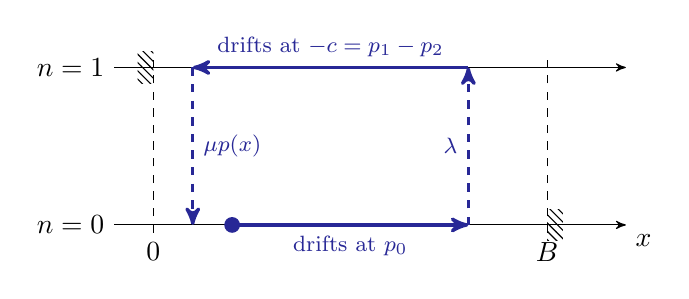
\begin{tikzpicture}
    \draw[->] (-0.5,-1) node[anchor=east] {$n=0$} -- (6,-1) node[below right] {$x$};
    \draw[->] (-0.5,1) node[anchor=east] {$n=1$} -- (6,1);
    \draw[dashed] (0,-1.1) node[below] {$0$} -- (0,1.1);
    \draw[dashed] (5,-1.1) node[below] {$B$} -- (5,1.1);

    %barriers
    \fill[pattern=north west lines] (5,-1.2) rectangle ++(.2,.4); 
    \fill[pattern=north west lines] (0,.8) rectangle ++(-.2,.4); 

    \draw[very thick,azulcito,->] (1,-1) --node[midway,below] {\footnotesize drifts at $p_0$} (4,-1);
    \draw[very thick,azulcito,->] (4,1) --node[midway,above] {\footnotesize drifts at $-c=p_1-p_2$} (0.5,1);
    \node[azulcito, fill=azulcito, circle, minimum size = .2cm, inner sep=0pt] at (1,-1) {};
    
    \draw[very thick, azulcito, dashed, ->] (4,-1) -- node[midway,anchor=east] {\footnotesize $\lambda$} (4,1);
    \draw[very thick, azulcito, dashed, ->] (0.5,1) -- node[midway,anchor=west] {\footnotesize $\mu p(x)$} (0.5,-1);
  \end{tikzpicture}
  \end{center}
  \caption{State space and system dynamics, showing a typical trajectory of $Z(t)$.}\label{fig:dynamics_single_server}
\end{figure}

Note that an arriving car always finds $x>0$ with probability one: during any idle
period the battery charges at rate $p_0>0$, and since the idle duration is
$\mathrm{Exp}(\lambda)$ (positive a.s.), the battery is strictly positive at every
arrival epoch. Consequently, $(n=0,x=0)$ has zero probability under any stationary
distribution, and we can restrict attention to $E' = \{0\}\times(0,B] \cup \{1\}\times[0,B]$.

% -------------------------------------------------------
\section{Single-Server in steady-state}
\label{sec:stationary}
% -------------------------------------------------------

\subsection{Stationary distribution}\label{ssec:stationary_dist}

Since $E$ is compact and $Z(t)$ is irreducible (every open rectangle
$\{n\}\times(a,b)$ is reachable with positive probability from any starting point, by
a combination of deterministic drift and Poisson events), the process is ergodic with a
unique stationary distribution $\pi$~\cite{MeynTweedie1993}.

We seek $\pi$ as a mixed measure of the form:
\begin{equation}
  \pi = f_0(x)dx + f_1(x)dx + \pi_{0,B}\delta_{(0,B)} + \pi_{1,0}\delta_{(1,0)}. 
  \label{eq:ansatz}
\end{equation}
Here $f_n(x)$, are the interior densities and $\pi_{0,B}, \pi_{1,0} \geq 0$ are point
masses at the corners where the flow accumulates: $x=B$ in mode~$0$ (since $r(0,\cdot)=p_0>0$)
and $x=0$ in mode~$1$ (since $r(1,\cdot)=-c<0$). The other two corners should carry no atoms since flow arriving on them is immediately carried into the interior by the flow (cf. Figure \ref{fig:dynamics_single_server}).

Substituting this form into $\int \mathcal{A}\psi\,d\pi = 0$ and using eqs. \eqref{eq:generator}, the
stationarity condition $\int \mathcal{A}\psi\,d\pi = 0$ for all $\psi \in \mathcal{D}(\mathcal{A})$ yields the following balance equations for the interior densities:
\begin{subequations}\label{eq:balance}
  \begin{align}
  p_0\, f_0'(x) &= -\lambda\, f_0(x) + \mu p_2\, f_1(x), \label{eq:E0} \\
  -c\, f_1'(x)  &= \phantom{-}\lambda\, f_0(x) - \mu p_2\, f_1(x). \label{eq:E1}
  \end{align}

As for the atoms, we obtain the following \emph{boundary flux equations}, obtained by flux conservation at each boundary
point. At $x=0$ in mode $1$, the inward flow $c\,f_1(0^+)$ feeds the atom $\pi_{1,0}$, which
drains via departures at rate $\mu p_1$:
\begin{equation}
  c\,f_1(0^+) = \mu p_1\,\pi_{1,0}. \label{eq:B1}
\end{equation}
Similarly, at $x=B$ in mode $0$, the inward flow $p_0\,f_0(B^-)$ feeds the atom $\pi_{0,B}$,
which drains via arrivals at rate $\lambda$:
\begin{equation}
  p_0\,f_0(B^-) = \lambda\,\pi_{0,B}. \label{eq:B2}
\end{equation}
Finally, at $(n,x)=(0,0)$, mass arriving from departures at rate $\mu p_1$ must immediately be carried at rate $p_0$ into the interior (no atom), yielding:
\begin{equation}
  p_0\,f_0(0^+) = \mu p_1\,\pi_{1,0}. \label{eq:B0}
\end{equation}
And finally by a similar argument, at $(n,x)=(1,B)$
\begin{equation}
  c\,f_1(B^-) = \lambda\,\pi_{0,B}. \label{eq:B3}
\end{equation}
\end{subequations}
Equations \eqref{eq:balance} provide the global balance equations for our system, which coupled with the normalization condition $\int_0^B (f_0 + f_1)\,dx + \pi_{0,B} + \pi_{1,0} = 1$ defines the steady-state distribution. We can now state the main result of this section.

\begin{theorem} \label{thm:stationary}
Let $\theta := \mu p_2/c - \lambda/p_0$. The unique stationary distribution of $Z(t)$ has the form~\eqref{eq:ansatz} with
\begin{subequations}\label{eq:steady_state}
\begin{equation}
  f_0(x) = \frac{e^{\theta x}}{K}, \qquad
  f_1(x) = \frac{p_0}{c}\cdot\frac{e^{\theta x}}{K}, \qquad x \in (0,B),
  \label{eq:densities}
\end{equation}
\begin{equation}
  \pi_{1,0} = \frac{p_0}{\mu p_1\, K}, \qquad
  \pi_{0,B} = \frac{p_0\,e^{\theta B}}{\lambda\, K},
  \label{eq:atoms}
\end{equation}
and the normalization constant is
\begin{equation}
  K = \frac{p_0+c}{c}\cdot\frac{e^{\theta B}-1}{\theta}
    + \frac{p_0}{\mu p_1} + \frac{p_0\,e^{\theta B}}{\lambda},
  \label{eq:K}
\end{equation}
\end{subequations}
with the convention $(e^{\theta B}-1)/\theta = B$ when $\theta = 0$.
\end{theorem}

\begin{proof}
Adding \eqref{eq:E0}, \eqref{eq:E1} gives $\frac{d}{dx}[p_0 f_0 - c f_1] = 0$, so $p_0 f_0 - c f_1$ is constant on $(0,B)$. Equations \eqref{eq:B1} and \eqref{eq:B0} together give $p_0 f_0(0^+) = c f_1(0^+)$, so the constant is zero. Therefore, $f_1(x) = (p_0/c)\,f_0(x)$ for all $x \in (0,B)$. Substituting this condition into \eqref{eq:E0} yields a first order differential equation for $f_0$, which accounting for the definition of $\theta$ is simply $f_0'(x) = \theta\, f_0(x)$. We conclude that $f_0$ (and thus also $f_1$) is exponential: $f_0(x) = f_0(0^+)\,e^{\theta x}$. With this expression, the atoms follow directly from \eqref{eq:B2}, \eqref{eq:B0}, and \eqref{eq:B3} is automatically satisfied, confirming consistency. Setting $f_0(0^+) = 1/K$ and imposing normalization
determines $K$ as in \eqref{eq:K}.
\end{proof}

The parameter $\theta$ has a physical interpretation: define the offered load of the system $\rho:=\lambda/\mu$, i.e. the average external power request. Consider now a single idle-busy cycle in the absence of battery boundaries: the battery
charges at rate $p_0$ during the idle period (mean duration $1/\lambda$) and discharges
at rate $c$ during the busy period with mean duration $1/(\mu p_2)$. Then, the expected net
battery change per cycle is therefore $\Delta := \frac{p_0}{\lambda} - \frac{c}{\mu p_2}$. It is easy to see that $\theta$ has the same sign as $\Delta$, in particular:
\begin{equation*}
  \theta > 0 \Leftrightarrow \rho < \frac{p_0p_2}{c} = \frac{p_0 p_2}{p_2-p_1}
\end{equation*}
This corresponds to a \emph{lightly loaded} station, where the battery gains energy on average on each cycle and thus tends to fill, concentrating its mass towards $x=B$. When $\rho > p_0 p_2/c$, we are in the \emph{highly loaded} regime, $\theta < 0$, the battery tends to drain and mass concentrates near $x = 0$, where a significant fraction of service occurs at the slow
rate $p_1$. When $\theta = 0$ the battery neither drains nor fills on average and stationary density is uniform on $(0, B)$.

\subsection{Performance metrics}\label{ssec:metrics}

We now derive key performance metrics directly from Theorem~\ref{thm:stationary}. We begin by computing the blocking probability, which, by the PASTA property, equals the stationary probability the charger is busy:
\begin{equation}
  P_B = \int_0^B f_1(x)\,dx + \pi_{1,0}
      = \frac{p_0}{K}\left(\frac{e^{\theta B}-1}{c\,\theta} + \frac{1}{\mu p_1}\right).
  \label{eq:PB}
\end{equation}
Note that this probability is also the probability that the charger is working. As $B \to 0$, $P_B \to \rho/(\rho + p_1)$, the blocking probability of an $M/M/1/1$ queue at rate $p_1$, since cars can only be served from the grid. Conversely, if the battery is large, as $B \to \infty$ we distinguish two cases: in the lightly loaded regime, $\theta > 0$ and $P_B \to \rho/(\rho + p_2)$, corresponding to service always at the fast rate $p_2$ because the battery can cope with the load and the system operates most of the time in fast charging. However, if the system is highly loaded ($\theta < 0$), $P_B$ converges to a value strictly between these two limits even as $B \to \infty$, reflecting that the system operates \emph{partly in both charging regimes} because the battery regularly depletes.

We now focus on the mean service time. Since there is at most one car in service, $E[N] = P_B$. By Little's law applied to admitted customers, $\lambda(1-P_B)E[T] = P_B$, so the mean service time of an admitted car is:
\begin{equation}
  \mathbb{E}[T] = \frac{P_B}{\lambda(1-P_B)}
  = \frac{1}{1 + \frac{\lambda B}{p_0}}\left(\frac{e^{\theta B}-1}{c\theta} + \frac{1}{\mu p_1}\right).
  \label{eq:ET}
\end{equation}
A more meaningful quantity is the \emph{average slowdown}, which we define as $E[T]$ normalized by the average service time in a system that operates at the fast rate $p_2$ permanently, which is given by:
\begin{equation}\label{eq:avg_slowdown}
  \bar{S} := \frac{\mu p_2\, \mathbb{E}[T]}{\mathbb{E}[Y]} = \frac{\mu p_2}{1 + \frac{\lambda B}{p_0}}\left(\frac{e^{\theta B}-1}{c\theta} + \frac{1}{\mu p_1}\right).
\end{equation}

A final quantity of interest is the \emph{slowdown factor}, measuring service
degradation relative to ideal fast charging:
\begin{equation}
  S(y) := \frac{\mathbb{E}[T \mid Y=y]}{y/p_2} \geq 1.
\end{equation}
The key quantity is $x_y := cy/p_2$, the battery level that would be exactly depleted
by demand $y$: if admitted at $x \geq x_y$ the car completes in Phase~1; if $x < x_y$
the battery depletes and Phase~2 is needed. This gives the compact formula
\begin{equation}
  T(x,y) = \frac{y}{p_2} + \frac{(x_y - x)^+}{p_1},
  \label{eq:Txy}
\end{equation}
so that $S(y) = 1 + (p_2/(p_1 y))\,\mathbb{E}[(x_y - x)^+]$, where the expectation
is over the admitted battery level. The threshold $x^* = p_2 B/c$ is the demand
at which even a full battery is exactly depleted; demands with $y < x^*$ (i.e.\
$x_y < B$) may complete in Phase~1, while $y \geq x^*$ always triggers Phase~2.

\begin{proposition}\label{prop:slowdown}
Let $x_y = cy/p_2$ and $K(1-P_B) = (e^{\theta B}-1)/\theta + p_0 e^{\theta B}/\lambda$.
For $y < p_2 B/c$:
\begin{equation}
  S(y) = 1 + \frac{c\,(e^{\theta x_y}-1-\theta x_y)}{p_1\,y\,\theta^2\,K(1-P_B)}.
  \label{eq:Sy1}
\end{equation}
For $y \geq p_2 B/c$:
\begin{equation}
  S(y) = \frac{p_2}{p_1} - \frac{p_2 B}{p_1\,y}
       + \frac{p_2\,(e^{\theta B}-1-\theta B)}{p_1\,y\,\theta^2\,K(1-P_B)}.
  \label{eq:Sy2}
\end{equation}
In both cases $S(y)\geq 1$, $S(y)\to 1$ as $y\to 0$ or $B\to\infty$,
and $S(y)\to p_2/p_1$ as $y\to\infty$ or $B\to 0$.
\end{proposition}
The proof is in Appendix~\ref{app:slowdown}.


\subsection{Optimal battery regime}\label{ssec:optimal_regime}

For practical battery health it is desirable to charge the battery \emph{slowly}, and to keep it \emph{cycling}
continuously rather than maintaining it fully charged or fully depleted for long periods. The stationary distribution of Theorem~\ref{thm:stationary} reveals a natural design criterion that achieves both goals simultaneously: namely control the value of the idle recharge rate $p_0$ to aim for the balanced regime where $\theta=0$ and the battery is kept most of the time in $(0,B)$ and not the boundaries.

To analyze this, we first introduce the following definitions. Let $\alpha = p_2/p_1 >1$ be the \emph{speed-up ratio} of fast vs. slow charging. Let $\beta = \mu B p_2 / c$ be the \emph{normalized battery capacity}, the ratio between the battery drain time and the average fast recharge session duration, i.e. how many full fast-charge sessions the battery can sustain before depleting. Finally, define the \emph{normalized load}
$\tilde\rho = \rho/p_2 = \lambda/(\mu p_2)$.

We aim for the uniform stationary density achieved when $\theta=0$. Setting $\theta = \mu p_2/c - \lambda/p_0=0$ uniquely determines the idle recharge rate as:
\begin{equation}
  p_0^* = \frac{\lambda c}{\mu p_2} = \tilde\rho\, c.
  \label{eq:p0star}
\end{equation}
The constraint $p_0^* \leqslant p_1$ requires then:
\begin{equation}
  \tilde\rho \leqslant \frac{p_1}{c} = \frac{1}{\alpha - 1} \; \Longleftrightarrow \; \rho \leqslant \rho_{\max} = \frac{p_1 p_2}{c}.
  \label{eq:rhomax}
\end{equation}
Below this threshold the operator can minimize battery stress by throttling down the idle recharge rate (slower recharge) and achieve the uniform regime. Above it, $\theta < 0$ regardless of $p_0$ and the battery drains in steady state.

Setting $\theta=0$ and $p_0 = p_0^*$ in the expressions for $K$ and $P_B$, one finds a simple form for the average slowdown in terms of the normalized battery capacity:
\begin{equation}
  \bar{S} = \frac{\alpha + \beta}{\beta + 1}.
  \label{eq:Sbar_beta}
\end{equation}
Remarkably, this depends only on $\alpha$ and $\beta$ and not on the load. This is very useful from a design perspective since \emph{the same design} works across all (feasible) loads $\rho<\rho_{\max}$, and decreases from $\alpha=p_2/p_1$ at $\beta\to 0$ (no battery) to $1$ at $\beta\to\infty$. Setting a target slowdown $\bar{S}_0 \in (1,\alpha)$ we get:
\begin{equation}
  \beta^* = \frac{\alpha - \bar{S}_0}{\bar{S}_0 - 1} \; \Longleftrightarrow \; B^* = \frac{c}{\mu p_2}\frac{\alpha - \bar{S}_0}{\bar{S}_0 - 1}.
  \label{eq:Bstar}
\end{equation}
Finally the blocking probability becomes:
\begin{equation}
  P_B = \frac{\tilde\rho\bar{S}_0}{1+\tilde\rho\bar{S}_0} = \frac{\tilde\rho(\alpha + \beta)}{\beta + 1 + \tilde\rho(\alpha + \beta)}.
  \label{eq:PB_opt}
\end{equation}
This has the form of an $M/M/1/1$ blocking formula with effective load
$\tilde\rho\bar{S}$. Unlike $\bar{S}$, the blocking probability depends on $\tilde\rho$, as expected.

\begin{figure}[t]
\centering
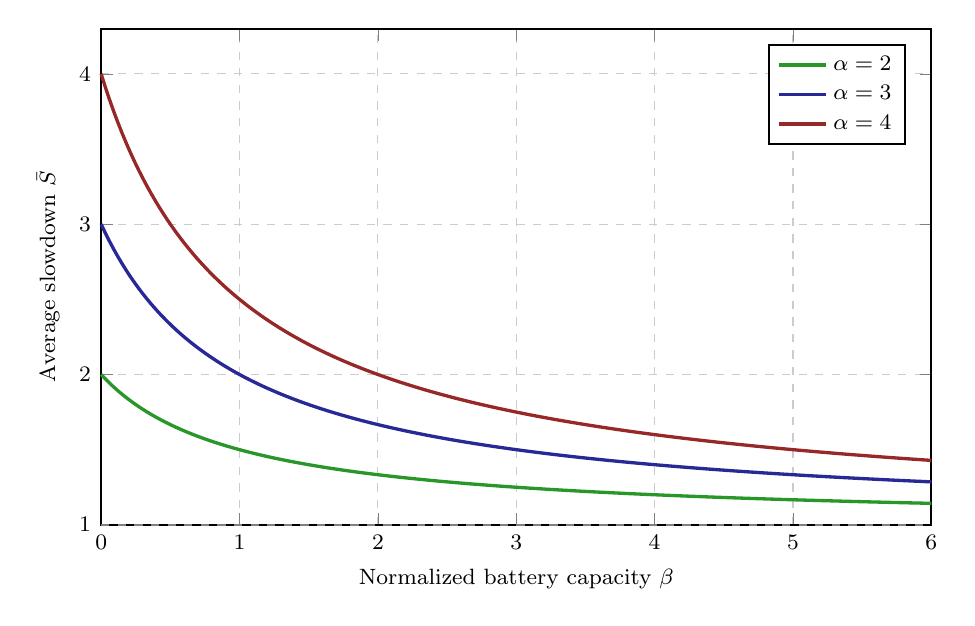
\begin{tikzpicture}
\begin{axis}[
  width=\columnwidth,
  height=0.65\columnwidth,
  xlabel={Normalized battery capacity $\beta$},
  ylabel={Average slowdown $\bar{S}$},
  xmin=0, xmax=6,
  ymin=1, ymax=4.3,
  xtick={0,1,2,3,4,5,6},
  ytick={1,2,3,4},
  yticklabels={$1$,$2$,$3$,$4$},
  grid=both,
  grid style={dashed,gray!40},
  thick,
  legend pos=north east,
  legend style={font=\footnotesize},
  clip=false,
]
\addplot[color=verdecito, very thick, domain=0:6, samples=200]
  {(x+2)/(x+1)};
\addlegendentry{$\alpha=2$}
\addplot[color=azulcito, very thick, domain=0:6, samples=200]
  {(x+3)/(x+1)};
\addlegendentry{$\alpha=3$}
\addplot[color=rojito, very thick, domain=0:6, samples=200]
  {(x+4)/(x+1)};
\addlegendentry{$\alpha=4$}
\addplot[dashed, gray, domain=0:6] {1};
\end{axis}
\end{tikzpicture}
\caption{Average slowdown $\bar{S}$ in the optimal battery regime as a function of normalized capacity $\beta = \mu B p_2/c$, for
three values of the speed-up ratio $\alpha = p_2/p_1$.}
\label{fig:Sbar}
\end{figure}

% -------------------------------------------------------
\section{Numerical Results}
\label{sec:sims}
% -------------------------------------------------------

We illustrate the theoretical results through event-driven simulations of the
single-server system. We set $p_2 = 150\,\unit{\kilo\watt}$, a typical DC fast
charger output, and $p_1 = 60\,\unit{\kilo\watt}$, representative of a medium-sized
grid connection; this gives $c = 90\,\unit{\kilo\watt}$ and $\alpha = p_2/p_1 = 2.5$.
For the energy demand distribution, large-scale data from the US
Department of Energy reports an average of 22 kWh per paid DC fast charging
session~\cite{NREL2023}, consistent with a partial top-up rather than a
full charge. We use $1/\mu = 20\,\unit{\kilo\watt\hour}$, giving a mean fast-charge
session duration of $1/(\mu p_2) = 20/150 \approx 8\,\unit{\minute}$.

We target an arrival rate of $\lambda = 3$ cars/h and aim to operate in the optimal
battery regime ($\theta = 0$), which requires $p_0^* = \tilde\rho c = (3/7.5)\times
90 = 36\,\unit{\kilo\watt}$ and is feasible since $\tilde\rho = 0.4 < 1/(\alpha-1)
= 0.667$. We size the battery to achieve an average slowdown of $\bar{S}_0 = 1.2$,
i.e.\ 20\% above the ideal fast-charging time. From~\eqref{eq:Bstar},
$\beta^* = (\alpha-\bar{S}_0)/(\bar{S}_0-1) = 1.3/0.2 = 6.5$, giving
$B^* = \beta^* c/(\mu p_2) = 6.5 \times 90/7.5 = 78\,\unit{\kilo\watt\hour}$.
As a sanity check, a car with mean demand $20\,\unit{\kilo\watt\hour}$ charging
at the slow rate $p_1 = 60\,\unit{\kilo\watt}$ would take $20\,\unit{\minute}$;
the design target of $\bar{S}=1.2$ corresponds to a mean service time of
$8 \times 1.2 = 9.6\,\unit{\minute}$, a modest 1.6-minute penalty. The resulting
system parameters are summarized in Table~\ref{tab:params}.

\begin{table}[t]
  \centering
  \caption{System parameters used in the numerical study.}
  \label{tab:params}
  \begin{tabular}{llr}
    \hline
    Parameter & Symbol & Value \\
    \hline
    Fast charging rate   & $p_2$        & $150\,\unit{\kilo\watt}$ \\
    Grid connection      & $p_1$        & $60\,\unit{\kilo\watt}$ \\
    Speed-up ratio       & $\alpha$     & $2.5$ \\
    Mean energy demand   & $1/\mu$      & $20\,\unit{\kilo\watt\hour}$ \\
    Arrival rate         & $\lambda$    & $3\,\text{cars/h}$ \\
    Idle recharge rate   & $p_0^*$      & $36\,\unit{\kilo\watt}$ \\
    Battery capacity     & $B^*$        & $78\,\unit{\kilo\watt\hour}$ \\
    Norm.\ battery cap.\ & $\beta^*$    & $6.5$ \\
    Target slowdown      & $\bar{S}_0$  & $1.2$ \\
    \hline
  \end{tabular}
\end{table}

To illustrate the three battery regimes, we fix the design parameters and vary the
arrival rate: $\lambda = 2$ (lightly loaded, $\theta > 0$), $\lambda = 3$ (optimal,
$\theta = 0$), and $\lambda = 4$ (heavily loaded, $\theta < 0$). Figure~\ref{fig:paths}
shows a sample path of $x(t)$ for each case. For $\lambda=2$ the battery drifts
toward $B$ and spends long periods near full; for $\lambda=4$ it drains toward zero
and service frequently degrades to the slow rate; for $\lambda=3$ it oscillates
freely across $(0,B)$ without dwelling at either boundary, consistent with the
uniform stationary density predicted by Theorem~\ref{thm:stationary}.

\begin{figure}[t]
  \centering
  % placeholder: three sample paths
  \caption{Sample paths of $x(t)$ for $\lambda = 2$ ($\theta>0$, top),
  $\lambda = 3$ ($\theta=0$, middle), and $\lambda = 4$ ($\theta<0$, bottom).}
  \label{fig:paths}
\end{figure}

We now focus on the design case $\lambda=3$ to validate the analytical formulas.
Figure~\ref{fig:hist} shows the empirical stationary distribution of $x$, which
closely matches the uniform density $1/B$ of Theorem~\ref{thm:stationary} at $\theta=0$.

\begin{figure}[t]
  \centering
  % placeholder: histogram vs uniform density
  \caption{Empirical stationary distribution of $x$ at $\lambda=3$ (histogram)
  vs.\ the uniform density $1/B$ (dashed).}
  \label{fig:hist}
\end{figure}

Table~\ref{tab:metrics} compares analytical and simulated values of $P_B$ and
$\bar{S}$. The analytical values follow from~\eqref{eq:PB_opt} and~\eqref{eq:Sbar_beta}.

\begin{table}[t]
  \centering
  \caption{Analytical vs.\ simulated performance metrics at $\lambda=3$, $\theta=0$.}
  \label{tab:metrics}
  \begin{tabular}{lcc}
    \hline
    Metric & Analytical & Simulated \\
    \hline
    $P_B$    & $0.324$ & \\
    $\bar{S}$ & $1.200$ & \\
    \hline
  \end{tabular}
\end{table}

Finally, Figure~\ref{fig:slowdown} shows the slowdown factor $S(u)$ as a function
of normalized demand $u = y/x^*$, validating Proposition~\ref{prop:slowdown}.
Cars with $u < 1$ may complete in Phase~1 and experience little slowdown;
those with $u \geq 1$ always exhaust the battery and suffer a slowdown approaching
$\alpha = 2.5$ for large demands.

\begin{figure}[t]
\centering
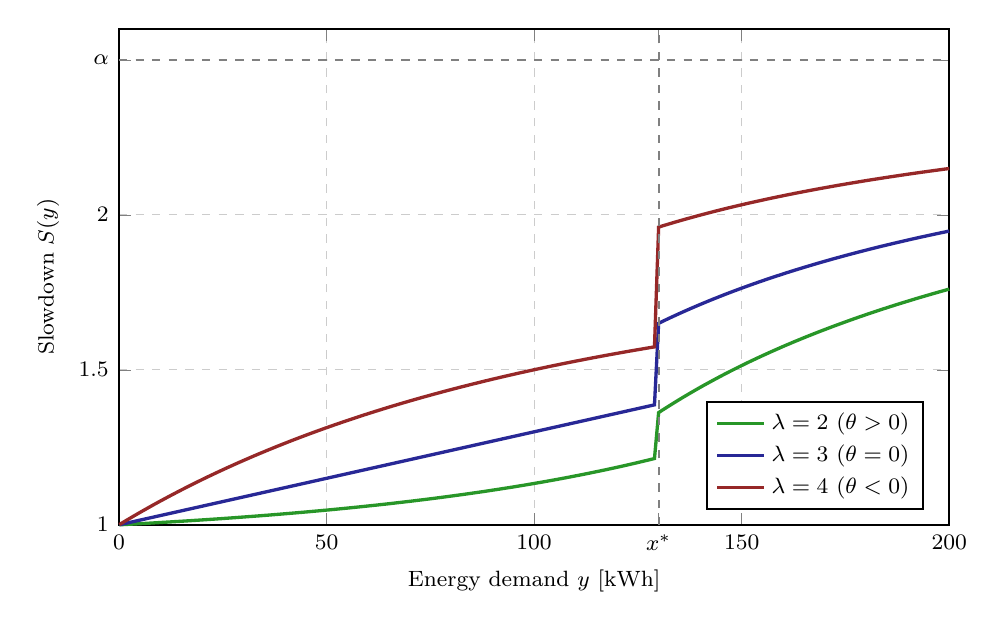
\begin{tikzpicture}
\begin{axis}[
  width=\columnwidth,
  height=0.65\columnwidth,
  xlabel={Energy demand $y$ [kWh]},
  ylabel={Slowdown $S(y)$},
  xmin=0, xmax=200,
  ymin=1, ymax=2.6,
  xtick={0,50,100,130,150,200},
  xticklabels={$0$,$50$,$100$,$x^*$,$150$,$200$},
  ytick={1,1.5,2,2.5},
  yticklabels={$1$,$1.5$,$2$,$\alpha$},
  grid=both,
  grid style={dashed,gray!40},
  thick,
  legend pos=south east,
  legend style={font=\footnotesize},
  clip=false,
]
\addplot[color=verdecito, very thick] coordinates {(0.1,1.0001) (0.2,1.0001) (0.3,1.0002) (0.4,1.0003) (0.5,1.0004) (0.6,1.0004) (0.7,1.0005) (0.8,1.0006) (0.9,1.0006) (1.0,1.0007) (1.1,1.0008) (1.2,1.0009) (1.3,1.0009) (1.4,1.0010) (1.5,1.0011) (1.6,1.0011) (1.7,1.0012) (1.8,1.0013) (1.9,1.0014) (2.0,1.0014) (2.1,1.0015) (2.2,1.0016) (2.3,1.0016) (2.4,1.0017) (2.5,1.0018) (2.6,1.0019) (2.7,1.0019) (2.8,1.0020) (2.9,1.0021) (3.0,1.0022) (3.1,1.0022) (3.2,1.0023) (3.3,1.0024) (3.4,1.0024) (3.5,1.0025) (3.6,1.0026) (3.7,1.0027) (3.8,1.0027) (3.9,1.0028) (4.0,1.0029) (4.1,1.0030) (4.2,1.0030) (4.3,1.0031) (4.4,1.0032) (4.5,1.0033) (4.6,1.0033) (4.7,1.0034) (4.8,1.0035) (4.9,1.0036) (6.0,1.0044) (7.0,1.0051) (8.0,1.0059) (9.0,1.0067) (10.0,1.0075) (11.0,1.0083) (12.0,1.0091) (13.0,1.0099) (14.0,1.0107) (15.0,1.0115) (16.0,1.0124) (17.0,1.0132) (18.0,1.0141) (19.0,1.0149) (20.0,1.0158) (21.0,1.0167) (22.0,1.0176) (23.0,1.0185) (24.0,1.0194) (25.0,1.0203) (26.0,1.0213) (27.0,1.0222) (28.0,1.0232) (29.0,1.0242) (30.0,1.0252) (31.0,1.0262) (32.0,1.0272) (33.0,1.0282) (34.0,1.0292) (35.0,1.0303) (36.0,1.0313) (37.0,1.0324) (38.0,1.0335) (39.0,1.0346) (40.0,1.0357) (41.0,1.0368) (42.0,1.0379) (43.0,1.0391) (44.0,1.0402) (45.0,1.0414) (46.0,1.0426) (47.0,1.0438) (48.0,1.0450) (49.0,1.0462) (50.0,1.0475) (51.0,1.0487) (52.0,1.0500) (53.0,1.0513) (54.0,1.0526) (55.0,1.0539) (56.0,1.0553) (57.0,1.0566) (58.0,1.0580) (59.0,1.0594) (60.0,1.0608) (61.0,1.0622) (62.0,1.0636) (63.0,1.0651) (64.0,1.0665) (65.0,1.0680) (66.0,1.0695) (67.0,1.0711) (68.0,1.0726) (69.0,1.0742) (70.0,1.0757) (71.0,1.0773) (72.0,1.0790) (73.0,1.0806) (74.0,1.0823) (75.0,1.0839) (76.0,1.0856) (77.0,1.0874) (78.0,1.0891) (79.0,1.0909) (80.0,1.0927) (81.0,1.0945) (82.0,1.0963) (83.0,1.0981) (84.0,1.1000) (85.0,1.1019) (86.0,1.1038) (87.0,1.1058) (88.0,1.1077) (89.0,1.1097) (90.0,1.1118) (91.0,1.1138) (92.0,1.1159) (93.0,1.1180) (94.0,1.1201) (95.0,1.1222) (96.0,1.1244) (97.0,1.1266) (98.0,1.1288) (99.0,1.1311) (100.0,1.1334) (101.0,1.1357) (102.0,1.1380) (103.0,1.1404) (104.0,1.1428) (105.0,1.1452) (106.0,1.1477) (107.0,1.1502) (108.0,1.1527) (109.0,1.1553) (110.0,1.1579) (111.0,1.1605) (112.0,1.1632) (113.0,1.1658) (114.0,1.1686) (115.0,1.1713) (116.0,1.1741) (117.0,1.1769) (118.0,1.1798) (119.0,1.1827) (120.0,1.1856) (121.0,1.1886) (122.0,1.1916) (123.0,1.1947) (124.0,1.1978) (125.0,1.2009) (126.0,1.2041) (127.0,1.2073) (128.0,1.2105) (129.0,1.2138) (130.0,1.3620) (131.0,1.3707) (132.0,1.3792) (133.0,1.3876) (134.0,1.3959) (135.0,1.4041) (136.0,1.4122) (137.0,1.4201) (138.0,1.4279) (139.0,1.4357) (140.0,1.4433) (141.0,1.4508) (142.0,1.4581) (143.0,1.4654) (144.0,1.4726) (145.0,1.4797) (146.0,1.4867) (147.0,1.4936) (148.0,1.5004) (149.0,1.5071) (150.0,1.5137) (151.0,1.5202) (152.0,1.5267) (153.0,1.5330) (154.0,1.5393) (155.0,1.5455) (156.0,1.5516) (157.0,1.5577) (158.0,1.5636) (159.0,1.5695) (160.0,1.5754) (161.0,1.5811) (162.0,1.5868) (163.0,1.5924) (164.0,1.5979) (165.0,1.6034) (166.0,1.6088) (167.0,1.6141) (168.0,1.6194) (169.0,1.6246) (170.0,1.6297) (171.0,1.6348) (172.0,1.6399) (173.0,1.6448) (174.0,1.6497) (175.0,1.6546) (176.0,1.6594) (177.0,1.6642) (178.0,1.6689) (179.0,1.6735) (180.0,1.6781) (181.0,1.6826) (182.0,1.6871) (183.0,1.6916) (184.0,1.6960) (185.0,1.7003) (186.0,1.7046) (187.0,1.7089) (188.0,1.7131) (189.0,1.7172) (190.0,1.7213) (191.0,1.7254) (192.0,1.7295) (193.0,1.7335) (194.0,1.7374) (195.0,1.7413) (196.0,1.7452) (197.0,1.7490) (198.0,1.7528) (199.0,1.7566) (200.0,1.7603)};
\addlegendentry{$\lambda=2$ ($\theta>0$)}
\addplot[color=azulcito, very thick] coordinates {(0.1,1.0003) (0.2,1.0006) (0.3,1.0009) (0.4,1.0012) (0.5,1.0015) (0.6,1.0018) (0.7,1.0021) (0.8,1.0024) (0.9,1.0027) (1.0,1.0030) (1.1,1.0033) (1.2,1.0036) (1.3,1.0039) (1.4,1.0042) (1.5,1.0045) (1.6,1.0048) (1.7,1.0051) (1.8,1.0054) (1.9,1.0057) (2.0,1.0060) (2.1,1.0063) (2.2,1.0066) (2.3,1.0069) (2.4,1.0072) (2.5,1.0075) (2.6,1.0078) (2.7,1.0081) (2.8,1.0084) (2.9,1.0087) (3.0,1.0090) (3.1,1.0093) (3.2,1.0096) (3.3,1.0099) (3.4,1.0102) (3.5,1.0105) (3.6,1.0108) (3.7,1.0111) (3.8,1.0114) (3.9,1.0117) (4.0,1.0120) (4.1,1.0123) (4.2,1.0126) (4.3,1.0129) (4.4,1.0132) (4.5,1.0135) (4.6,1.0138) (4.7,1.0141) (4.8,1.0144) (4.9,1.0147) (6.0,1.0180) (7.0,1.0210) (8.0,1.0240) (9.0,1.0270) (10.0,1.0300) (11.0,1.0330) (12.0,1.0360) (13.0,1.0390) (14.0,1.0420) (15.0,1.0450) (16.0,1.0480) (17.0,1.0510) (18.0,1.0540) (19.0,1.0570) (20.0,1.0600) (21.0,1.0630) (22.0,1.0660) (23.0,1.0690) (24.0,1.0720) (25.0,1.0750) (26.0,1.0780) (27.0,1.0810) (28.0,1.0840) (29.0,1.0870) (30.0,1.0900) (31.0,1.0930) (32.0,1.0960) (33.0,1.0990) (34.0,1.1020) (35.0,1.1050) (36.0,1.1080) (37.0,1.1110) (38.0,1.1140) (39.0,1.1170) (40.0,1.1200) (41.0,1.1230) (42.0,1.1260) (43.0,1.1290) (44.0,1.1320) (45.0,1.1350) (46.0,1.1380) (47.0,1.1410) (48.0,1.1440) (49.0,1.1470) (50.0,1.1500) (51.0,1.1530) (52.0,1.1560) (53.0,1.1590) (54.0,1.1620) (55.0,1.1650) (56.0,1.1680) (57.0,1.1710) (58.0,1.1740) (59.0,1.1770) (60.0,1.1800) (61.0,1.1830) (62.0,1.1860) (63.0,1.1890) (64.0,1.1920) (65.0,1.1950) (66.0,1.1980) (67.0,1.2010) (68.0,1.2040) (69.0,1.2070) (70.0,1.2100) (71.0,1.2130) (72.0,1.2160) (73.0,1.2190) (74.0,1.2220) (75.0,1.2250) (76.0,1.2280) (77.0,1.2310) (78.0,1.2340) (79.0,1.2370) (80.0,1.2400) (81.0,1.2430) (82.0,1.2460) (83.0,1.2490) (84.0,1.2520) (85.0,1.2550) (86.0,1.2580) (87.0,1.2610) (88.0,1.2640) (89.0,1.2670) (90.0,1.2700) (91.0,1.2730) (92.0,1.2760) (93.0,1.2790) (94.0,1.2820) (95.0,1.2850) (96.0,1.2880) (97.0,1.2910) (98.0,1.2940) (99.0,1.2970) (100.0,1.3000) (101.0,1.3030) (102.0,1.3060) (103.0,1.3090) (104.0,1.3120) (105.0,1.3150) (106.0,1.3180) (107.0,1.3210) (108.0,1.3240) (109.0,1.3270) (110.0,1.3300) (111.0,1.3330) (112.0,1.3360) (113.0,1.3390) (114.0,1.3420) (115.0,1.3450) (116.0,1.3480) (117.0,1.3510) (118.0,1.3540) (119.0,1.3570) (120.0,1.3600) (121.0,1.3630) (122.0,1.3660) (123.0,1.3690) (124.0,1.3720) (125.0,1.3750) (126.0,1.3780) (127.0,1.3810) (128.0,1.3840) (129.0,1.3870) (130.0,1.6500) (131.0,1.6565) (132.0,1.6629) (133.0,1.6692) (134.0,1.6754) (135.0,1.6815) (136.0,1.6875) (137.0,1.6934) (138.0,1.6993) (139.0,1.7050) (140.0,1.7107) (141.0,1.7163) (142.0,1.7218) (143.0,1.7273) (144.0,1.7326) (145.0,1.7379) (146.0,1.7432) (147.0,1.7483) (148.0,1.7534) (149.0,1.7584) (150.0,1.7633) (151.0,1.7682) (152.0,1.7730) (153.0,1.7778) (154.0,1.7825) (155.0,1.7871) (156.0,1.7917) (157.0,1.7962) (158.0,1.8006) (159.0,1.8050) (160.0,1.8094) (161.0,1.8137) (162.0,1.8179) (163.0,1.8221) (164.0,1.8262) (165.0,1.8303) (166.0,1.8343) (167.0,1.8383) (168.0,1.8423) (169.0,1.8462) (170.0,1.8500) (171.0,1.8538) (172.0,1.8576) (173.0,1.8613) (174.0,1.8649) (175.0,1.8686) (176.0,1.8722) (177.0,1.8757) (178.0,1.8792) (179.0,1.8827) (180.0,1.8861) (181.0,1.8895) (182.0,1.8929) (183.0,1.8962) (184.0,1.8995) (185.0,1.9027) (186.0,1.9059) (187.0,1.9091) (188.0,1.9122) (189.0,1.9153) (190.0,1.9184) (191.0,1.9215) (192.0,1.9245) (193.0,1.9275) (194.0,1.9304) (195.0,1.9333) (196.0,1.9362) (197.0,1.9391) (198.0,1.9419) (199.0,1.9447) (200.0,1.9475)};
\addlegendentry{$\lambda=3$ ($\theta=0$)}
\addplot[color=rojito, very thick] coordinates {(0.1,1.0008) (0.2,1.0016) (0.3,1.0024) (0.4,1.0032) (0.5,1.0040) (0.6,1.0049) (0.7,1.0057) (0.8,1.0065) (0.9,1.0073) (1.0,1.0081) (1.1,1.0089) (1.2,1.0097) (1.3,1.0105) (1.4,1.0113) (1.5,1.0121) (1.6,1.0129) (1.7,1.0137) (1.8,1.0145) (1.9,1.0153) (2.0,1.0161) (2.1,1.0169) (2.2,1.0176) (2.3,1.0184) (2.4,1.0192) (2.5,1.0200) (2.6,1.0208) (2.7,1.0216) (2.8,1.0224) (2.9,1.0232) (3.0,1.0240) (3.1,1.0247) (3.2,1.0255) (3.3,1.0263) (3.4,1.0271) (3.5,1.0279) (3.6,1.0287) (3.7,1.0294) (3.8,1.0302) (3.9,1.0310) (4.0,1.0318) (4.1,1.0325) (4.2,1.0333) (4.3,1.0341) (4.4,1.0349) (4.5,1.0356) (4.6,1.0364) (4.7,1.0372) (4.8,1.0380) (4.9,1.0387) (6.0,1.0471) (7.0,1.0547) (8.0,1.0622) (9.0,1.0696) (10.0,1.0769) (11.0,1.0841) (12.0,1.0913) (13.0,1.0983) (14.0,1.1053) (15.0,1.1123) (16.0,1.1191) (17.0,1.1259) (18.0,1.1326) (19.0,1.1392) (20.0,1.1458) (21.0,1.1523) (22.0,1.1587) (23.0,1.1650) (24.0,1.1713) (25.0,1.1775) (26.0,1.1837) (27.0,1.1897) (28.0,1.1958) (29.0,1.2017) (30.0,1.2076) (31.0,1.2134) (32.0,1.2192) (33.0,1.2249) (34.0,1.2306) (35.0,1.2361) (36.0,1.2417) (37.0,1.2471) (38.0,1.2526) (39.0,1.2579) (40.0,1.2632) (41.0,1.2685) (42.0,1.2737) (43.0,1.2788) (44.0,1.2839) (45.0,1.2889) (46.0,1.2939) (47.0,1.2988) (48.0,1.3037) (49.0,1.3085) (50.0,1.3133) (51.0,1.3180) (52.0,1.3227) (53.0,1.3273) (54.0,1.3319) (55.0,1.3365) (56.0,1.3409) (57.0,1.3454) (58.0,1.3498) (59.0,1.3542) (60.0,1.3585) (61.0,1.3627) (62.0,1.3670) (63.0,1.3711) (64.0,1.3753) (65.0,1.3794) (66.0,1.3835) (67.0,1.3875) (68.0,1.3915) (69.0,1.3954) (70.0,1.3993) (71.0,1.4032) (72.0,1.4070) (73.0,1.4108) (74.0,1.4145) (75.0,1.4182) (76.0,1.4219) (77.0,1.4255) (78.0,1.4291) (79.0,1.4327) (80.0,1.4362) (81.0,1.4397) (82.0,1.4432) (83.0,1.4466) (84.0,1.4500) (85.0,1.4534) (86.0,1.4567) (87.0,1.4600) (88.0,1.4633) (89.0,1.4665) (90.0,1.4698) (91.0,1.4729) (92.0,1.4761) (93.0,1.4792) (94.0,1.4823) (95.0,1.4853) (96.0,1.4884) (97.0,1.4914) (98.0,1.4943) (99.0,1.4973) (100.0,1.5002) (101.0,1.5031) (102.0,1.5059) (103.0,1.5088) (104.0,1.5116) (105.0,1.5144) (106.0,1.5171) (107.0,1.5199) (108.0,1.5226) (109.0,1.5252) (110.0,1.5279) (111.0,1.5305) (112.0,1.5331) (113.0,1.5357) (114.0,1.5383) (115.0,1.5408) (116.0,1.5433) (117.0,1.5458) (118.0,1.5483) (119.0,1.5507) (120.0,1.5531) (121.0,1.5555) (122.0,1.5579) (123.0,1.5603) (124.0,1.5626) (125.0,1.5649) (126.0,1.5672) (127.0,1.5695) (128.0,1.5718) (129.0,1.5740) (130.0,1.9603) (131.0,1.9645) (132.0,1.9685) (133.0,1.9725) (134.0,1.9765) (135.0,1.9803) (136.0,1.9842) (137.0,1.9879) (138.0,1.9916) (139.0,1.9953) (140.0,1.9989) (141.0,2.0024) (142.0,2.0060) (143.0,2.0094) (144.0,2.0128) (145.0,2.0162) (146.0,2.0195) (147.0,2.0228) (148.0,2.0260) (149.0,2.0292) (150.0,2.0323) (151.0,2.0354) (152.0,2.0385) (153.0,2.0415) (154.0,2.0444) (155.0,2.0474) (156.0,2.0503) (157.0,2.0532) (158.0,2.0560) (159.0,2.0588) (160.0,2.0615) (161.0,2.0643) (162.0,2.0669) (163.0,2.0696) (164.0,2.0722) (165.0,2.0748) (166.0,2.0774) (167.0,2.0799) (168.0,2.0824) (169.0,2.0849) (170.0,2.0873) (171.0,2.0897) (172.0,2.0921) (173.0,2.0945) (174.0,2.0968) (175.0,2.0991) (176.0,2.1014) (177.0,2.1036) (178.0,2.1059) (179.0,2.1081) (180.0,2.1103) (181.0,2.1124) (182.0,2.1145) (183.0,2.1166) (184.0,2.1187) (185.0,2.1208) (186.0,2.1228) (187.0,2.1248) (188.0,2.1268) (189.0,2.1288) (190.0,2.1308) (191.0,2.1327) (192.0,2.1346) (193.0,2.1365) (194.0,2.1384) (195.0,2.1402) (196.0,2.1421) (197.0,2.1439) (198.0,2.1457) (199.0,2.1475) (200.0,2.1492)};
\addlegendentry{$\lambda=4$ ($\theta<0$)}
\addplot[dashed, gray, domain=0:200] {2.5};
\draw[dashed, gray] (axis cs:130,1) -- (axis cs:130,2.6);
% empirical dots placeholder
\end{axis}
\end{tikzpicture}
\caption{Slowdown factor $S(y)$ from Proposition~\ref{prop:slowdown} for three
load regimes. The vertical dashed line marks $x^*=p_2B/c=130$ kWh (the demand that
exactly depletes a full battery); the horizontal dashed line marks $\alpha=p_2/p_1=2.5$.
Empirical estimates from simulation (dots) to be added.}
\label{fig:slowdown}
\end{figure}

% -------------------------------------------------------
\section{The Many-Server Case}
\label{sec:multiserver}
% -------------------------------------------------------

The single-server analysis extends naturally to $s \geq 1$ parallel chargers sharing
a battery buffer of capacity $B$ and a grid connection of rate $p_1$, operating as a
loss system. We set $p_0 = p_1$ for simplicity; the case $p_0 \neq p_1$ can be handled
with additional notation.

The state is $Z(t) = (n(t), x(t))$ with $n(t) \in \{0,\ldots,s\}$ and $x(t) \in [0,B]$.
With $p_0=p_1$ the net battery drift is $r_n = p_1 - np_2$ uniformly for all $n$:
the battery charges when $n \leq n^* := \lfloor p_1/p_2 \rfloor$ and drains when
$n > n^*$. Arrivals occur at rate $\lambda$ when $n<s$; departures at total rate
$n\mu p_2$ when $x>0$ and at rate $\mu p_1$ when $x=0$. The process is again an
ergodic PDMP by the same arguments as Section~\ref{sec:model}.

The stationary balance equations on $(0,B)$ take the form $R\,\mathbf{f}'(x) = Q\,\mathbf{f}(x)$,
where $\mathbf{f}(x) = (f_0(x),\ldots,f_s(x))^T$, $R = \mathrm{diag}(r_0,\ldots,r_s)$
is the diagonal drift matrix, and $Q$ is the $(s+1)\times(s+1)$ transition rate matrix
of the occupancy chain. When $p_2/p_1 \notin \mathbb{N}$, $R$ is invertible and
exponential solutions $\mathbf{f}(x) = \mathbf{a}\,e^{\theta x}$ require $(\theta,\mathbf{a})$
to be an eigenpair of $R^{-1}Q$. This pencil has $s+1$ eigenvalues, one of which is
always $\theta = 0$: setting $\theta=0$ gives $Q\mathbf{a}=0$, whose solution is the
Erlang-B stationary distribution $a_n = \rho^n/n!$. The general interior solution is
therefore a superposition of all $s+1$ exponential modes.

The boundary conditions provide exactly $s+1$ equations (two tridiagonal systems, one
at $x=B$ and one at $x=0$, coupled at $n=n^*$, plus normalization), which generically
determine all $s+1$ coefficients. In contrast with the single-server case, where the
decoupling property of Theorem~\ref{thm:stationary} reduces the solution to a single
mode, the full spectrum of the pencil $(Q,R)$ is generically needed for $s>1$.

Two open questions must be resolved before a complete solution can be stated: whether
the eigenvalues of $R^{-1}Q$ are always real, and whether the corresponding
coefficients are always positive — both necessary for $\mathbf{f}(x)$ to be a valid
density. We conjecture both hold, but proofs remain open. The complete matrix-analytic
treatment is the subject of ongoing work.


% -------------------------------------------------------
\section{Conclusions}
\label{sec:conclusions}
% -------------------------------------------------------

We have studied a battery-buffered EV fast charging station using the framework of
piecewise-deterministic Markov processes. For the single-server loss system we derived
the stationary distribution in closed form, establishing a decoupling property that
separates the battery level from the charger state in steady state, and obtained explicit
expressions for the blocking probability, mean charging time, and slowdown factor. We
identified an optimal battery regime ($\theta=0$) in which the average slowdown depends
only on hardware parameters and not on load, and derived explicit sizing formulas for
the battery capacity and recharge rate.

The many-server extension reveals a richer structure: the interior balance equations
take the form of a matrix ODE whose solutions are superpositions of the eigenmodes of
the pencil $(Q,R)$, and the boundary conditions couple two tridiagonal systems at each
boundary. This matrix-analytic treatment, as well as numerical illustrations of the
single-server performance metrics, are the subject of ongoing work.


\bibliographystyle{abbrv}
\bibliography{evcharging}

\appendix

\section{Proof of Proposition~\ref{prop:slowdown}}
\label{app:slowdown}

From~\eqref{eq:Txy}, $S(y) = 1 + (p_2/(p_1 y))\,\mathbb{E}[(x_y-x)^+]$,
where $x$ has the admitted distribution: density $e^{\theta x}/(K(1-P_B))$ on
$(0,B)$ and atom $\pi_{0,B}/(1-P_B)$ at $x=B$, with $\pi_{0,B}=p_0 e^{\theta B}/(\lambda K)$.
Since $(x_y-x)^+=0$ for $x\geq x_y$, only admitted levels $x<x_y$ contribute.
The fundamental integral needed is
\begin{equation}
  J(a) := \int_0^a (a-x)\,e^{\theta x}\,dx = \frac{e^{\theta a}-1-\theta a}{\theta^2},
  \label{eq:Ja}
\end{equation}
obtained by integration by parts.

\textit{Case~1: $y < p_2B/c$.} Here $x_y < B$, so the atom at $x=B$ satisfies
$B > x_y$ and contributes nothing to $(x_y-x)^+$. Thus
\[
  \mathbb{E}[(x_y-x)^+] = \frac{J(x_y)}{K(1-P_B)}.
\]
Substituting and using $x_y = cy/p_2$, so $p_2 J(x_y)/(p_1 y) = c J(x_y)/(p_1 x_y)$,
gives~\eqref{eq:Sy1}.

\textit{Case~2: $y \geq p_2B/c$.} Here $x_y \geq B$, so all interior levels and
the atom contribute. We compute
\begin{align*}
  \int_0^B(x_y-x)e^{\theta x}\,dx
  &= x_y\frac{e^{\theta B}-1}{\theta} - \frac{Be^{\theta B}}{\theta}
     + \frac{e^{\theta B}-1}{\theta^2} \\
  &= J(B) + (x_y-B)\frac{e^{\theta B}-1}{\theta},
\end{align*}
where the second equality uses $J(B) = (e^{\theta B}-1-\theta B)/\theta^2$.
Adding the atom contribution $\pi_{0,B}(x_y-B) = (p_0 e^{\theta B}/\lambda)(x_y-B)$:
\begin{equation*}
  \mathbb{E}[(x_y-x)^+]
  = \frac{J(B) + (x_y-B)\bigl[(e^{\theta B}-1)/\theta + p_0 e^{\theta B}/\lambda\bigr]}{K(1-P_B)}.
\end{equation*}
Since $(e^{\theta B}-1)/\theta + p_0 e^{\theta B}/\lambda = K(1-P_B)$, this simplifies to
\[
  \mathbb{E}[(x_y-x)^+] = \frac{J(B)}{K(1-P_B)} + (x_y - B).
\]
Therefore
\[
  S(y) = 1 + \frac{p_2}{p_1 y}\!\left[\frac{J(B)}{K(1-P_B)} + (x_y-B)\right].
\]
Since $p_2(x_y-B)/(p_1 y) = c/p_1 - p_2 B/(p_1 y)$, we get
$1 + c/p_1 - p_2 B/(p_1 y) = p_2/p_1 - p_2 B/(p_1 y)$, and substituting $J(B)$
yields~\eqref{eq:Sy2}.

The limits follow directly: as $y\to 0$, $J(x_y)\sim \theta^2 x_y^2/2 \to 0$
so $S\to 1$; as $y\to\infty$, Case~2 gives $S = p_2/p_1 - p_2 B/(p_1 y)+O(1/y)\to p_2/p_1$;
as $B\to\infty$, $K(1-P_B)\to\infty$ so $S\to 1$; as $B\to 0$, $x_y\geq B=0$ always
and $S = 1 + c/p_1 = p_2/p_1$. \qed



\end{document}


